\documentclass[14pt]{extarticle}
\usepackage{graphicx} %package to manage images
\usepackage{graphics}
\usepackage[utf8]{inputenc}
\graphicspath{ {./} }
\usepackage[utf8]{inputenc}
\usepackage{multirow}
\usepackage{hyperref}
\usepackage{cite}
\usepackage{natbib}
\title{ {\huge Performance Improvisation in Matrix Multiplication}}

\author{{\huge Vijay, Vedant} \\  \href{mailto:Vvijay1000@gmail.com}{cs1170388@iitd.ac.in} 
   \and {\huge Bansal, Shivam} \\  \href{mailto:cs1170376@iitd.ac.in}{cs1170376@iitd.ac.in} }
\date{17 February, 2019}
\begin{document}
\maketitle
\newpage
\section{Introduction}
The Report consists details of different approaches(i.e libraries) used to improve the performance of LeNet structure. It helps to fasten the code and improve accuracy as well. 
\section{Linear Algebra Libraries}
The main segment of LeNet algorithm which consumes time Convolution which solely depends on matrix multiplication. Direct Matrix multiplication by evaluation of each value proves out to be unacceptably slower for large number of values. Following are decribed the two improvement by usage of external libraries for C++ such as MKL and OpenBlas.
\subsection{MKL }
\cite{IntelMKL1}
Intel MKL greatly improves the performance of Basic Linear Algebra Subprograms (BLAS) and Linear Algebra Package (LAPACK) functions since it takes advantage of special features in the new generation of Intel processors that greatly speed up matrix operations. With Intel MKL, we don’t need to modify our source code to take advantage of new features of Intel processors. 
\subsection{OpenBlas \cite{OpenBLAS}}
BLAS is divided into three levels:
\begin{itemize}
\item Level 1 defines a set of linear algebra functions that operate on vectors only. These functions benefit from vectorization.
\item Level 2 functions are matrix-vector operations, e.g. some matrix-vector product. These functions could be implemented in terms of Level1 functions. However, you can boost the performance of this functions if you can provide a dedicated implementation that makes use of some multiprocessor architecture with shared memory.
\item Level 3 functions are operations like the matrix-matrix product. Again you could implement them in terms of Level2 functions. But Level3 functions perform O(N3) operations on O(N2) data. So if your platform has a cache hierarchy then you can boost performance if you provide a dedicated implementation that is cache optimized/cache friendly. The main boost of Level3 functions comes from cache optimization. This boost significantly exceeds the second boost from parallelism and other hardware optimizations. 
\end{itemize}
\section{Performance Comparision}
Following are three figures which depicts comparision between performance between OpenBlas and MKL library. It helps us understand the difference between two libraries by plotting time vs libarary curves for three sizes of Matrix mentioned below.
\newpage
\begin{figure}[t]
\centering
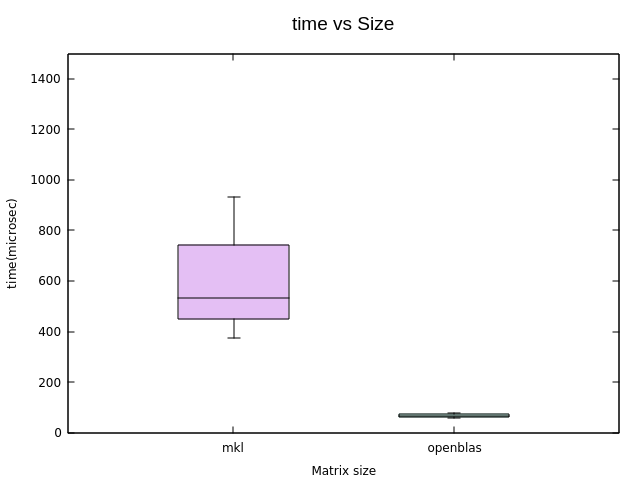
\includegraphics[width=16cm]{50x3.png}
\end{figure}
Size of matrix = 50 
\newpage
\begin{figure}[t]
\centering
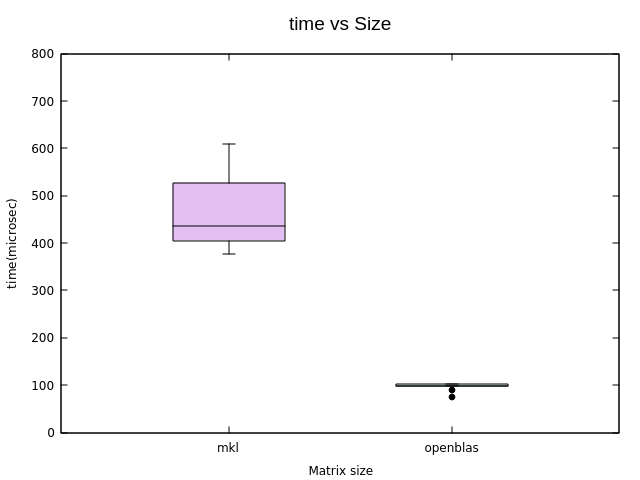
\includegraphics[width=16cm]{75x3.png}
\end{figure}
size of matrix = 75
\newpage
\begin{figure}[t]
\centering
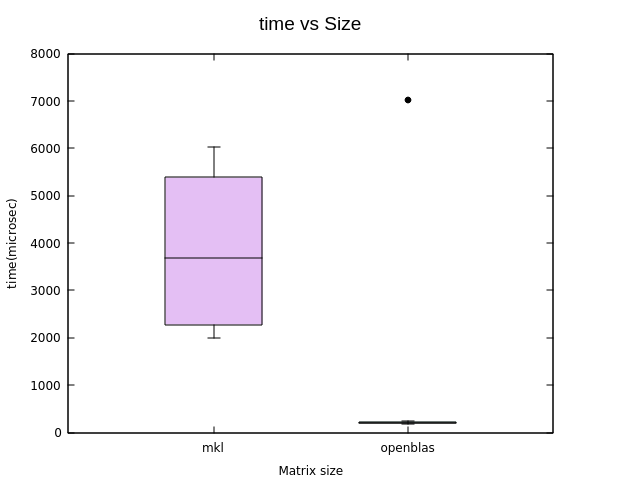
\includegraphics[width=16cm]{100x3.png}
\end{figure}
size of matrix =100
\newpage

% \resizebox{\columnwidth}{!}{}

The overall comparision of MKL and OpenBlas is written in next section along with Pthreads.
\section{Acceleration with Pthreads}
The work we did:
\begin{itemize}
\item We tried using 2 threads, 4 and 8 threads to increase the efficiency of the code. 
\item But increase in threads only lead to increase in run time. 
\item So we decided to go with MxN threads as we thought increase in threads must lead to decrease in runtime
\item It turned out that it was not the case as creating new threads also takes some time and the advantage of creating new thread must be more than the time taken to create one in order to decrease the runtime.
\end{itemize}
\newpage
\begin{figure}[t]
\centering
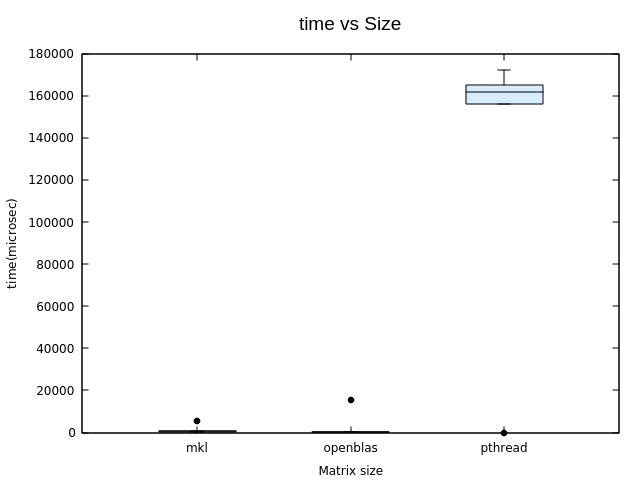
\includegraphics[width=16cm]{50x3withpthread.png}
\end{figure}
Size of matrix = 50 
\newpage
\begin{figure}[t]
\centering
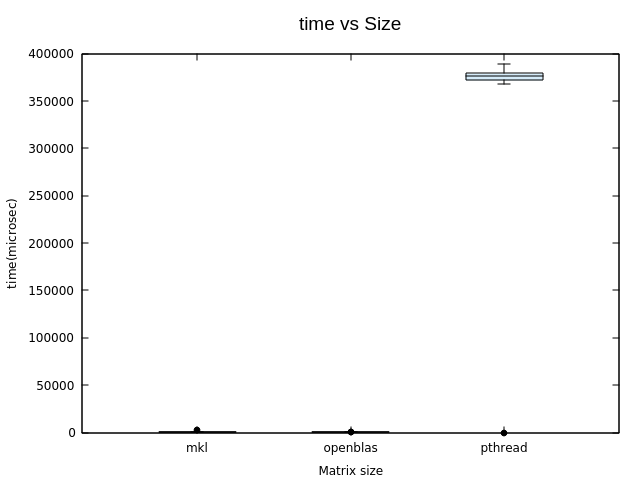
\includegraphics[width=16cm]{75x3withpthread.png}
\end{figure}
size of matrix = 75
\newpage
\begin{figure}[t]
\centering
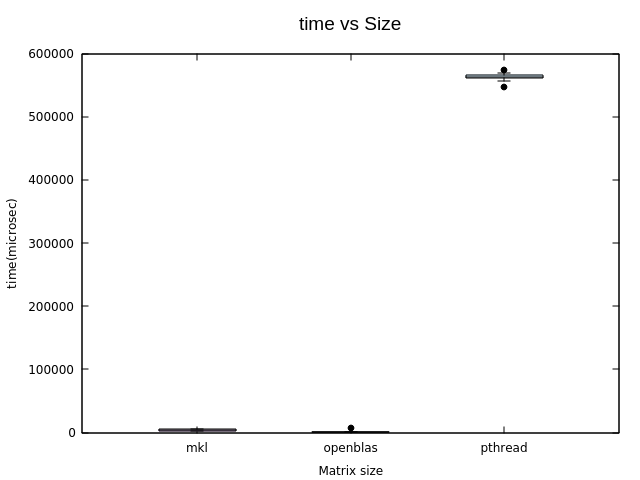
\includegraphics[width=16cm]{100x3withpthread.png}
\end{figure}
size of matrix =100
\newpage


Comparision between MKL, OpenBlas and Pthreads: \\
\begin{table}[h!]
\resizebox{\columnwidth}{!}{
\begin{tabular}{|l|l|l|l|l|l|l|l|}
\hline
\multirow{2}{*}{Matrix Size} & \multirow{2}{*}{Kernel Size} & \multicolumn{2}{l|}{Running Time- MKL} & \multicolumn{2}{l|}{Running Time- OpenBlas} & \multicolumn{2}{l|}{Running Time- Pthreads} \\ \cline{3-8} 
                             &                              & x                  & d                 & x                    & d                    & x                     & d                   \\ \hline
50x50                        & 3x3                          & 1066.3             & 1470.6            & 1621.7               & 4666.7               & 161993.3              & 4855.2              \\ \hline
75x75                        & 3x3                          & 656.5              & 606               & 99.2                 & 3.48                 & 377160.6              & 5564.1              \\ \hline
100x100                      & 3x3                          & 3964               & 1520.1            & 888.5                & 2045.8               & 563411                & 7112.5              \\ \hline
\end{tabular}
}
\end{table}
\\ x: Mean Time(in microsecond)
\\ d: Standard Deviation(in microsecond)
\section{Conclusion}
Time taken by MKL is less than OpenBlas is less than pthread. Pthread takes more time than others as we have used MxN threads and creating new thread is time consuming. 
MKL takes less time as we ran the code on an intel machine and MKL is optimized for intel processors whereas openblas is indifferent for the type of processors.
\bibliographystyle{unsrt}
%bibliography{plain}
\bibliography{report}

\end{document}
